\setcounter{section}{0}
\section{Lý thuyết}
\subsection{Khối lượng riêng}
Khối lượng riêng của một chất là khối lượng của một đơn vị thể tích chất đó:
$$\rho = \dfrac{m}{V}$$

Đơn vị của khối lượng riêng trong hệ SI là $\text{kg}/\text{m}^3$. Người ta cũng thường dùng đơn vị khối lượng riêng là $\text{g}/\text{cm}^3$.
$$1\text{ g}/\text{cm}^3= \dfrac{\SI{e-3}{\kilogram}}{(\SI{e-2}{\meter})^3}= 1000 \text{ kg}/\text{m}^3$$


\subsection{Áp lực và áp suất}
\subsubsection{Áp lực}
Áp lực của một vật lên một mặt phẳng là lực ép của vật tác dụng lên mặt phẳng theo phương vuông góc. Ví dụ: lực $\vec F_\text{N}$ ép lên mặt bàn theo phương vuông góc với mặt bàn được gọi là áp lực.
\begin{center}
	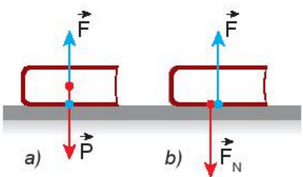
\includegraphics[scale=0.6]{../figs/G10-029-1}
\end{center}
\subsubsection{Áp suất}
Áp suất bằng áp lực chia cho diện tích bị ép.
$$p = \dfrac{F}{S}$$

Đơn vị của áp suất là pascal (Pa):
$$\SI{1}{Pa} = \SI{1}{N/m^2}$$

\subsection{Áp suất của chất lỏng}
\subsubsection{Nhắc lại về chất lỏng}
\begin{minipage}[l]{0.7\linewidth}
	Mật độ phân tử ở chất lỏng lớn gấp nhiều lần mật độ phân tử ở chất khí và nhỏ hơn mật độ phân tử trong chất rắn.
	
	Trong chất lỏng, mỗi phân tử tương tác với những phân tử khác ở gần. Nó dao động xung quanh một vị trí cân bằng tạm thời và từng lúc. Do tương tác, nó nhảy sang vị trí cân bằng mới và tiếp tục dao động xung quanh vị trí cân bằng mới này.
	
	Chất lỏng có thể tích riêng xác định nhưng không có hình dạng riêng xác định.
\end{minipage}
\begin{minipage}[r]{0.25\linewidth}
	\begin{flushright}
		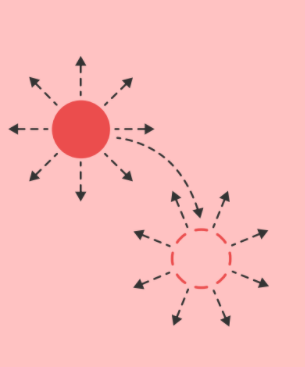
\includegraphics[scale=0.5,angle=90]{../figs/VN10-PH-46-L-0341-1.png}
	\end{flushright}
\end{minipage}
\subsubsection{Hiện tượng căng bề mặt của chất lỏng}

Hiện tượng căng bề mặt của chất lỏng là hiện tượng xảy ra tại bề mặt của chất lỏng, tại đó xuất hiện lực căng bề mặt có xu hướng giữ cho diện tích bề mặt của chất lỏng là nhỏ nhất.

Những lực kéo căng bề mặt chất lỏng được gọi là lực căng bề mặt của chất lỏng.

Lực căng bề mặt tác dụng lên một đoạn đường nhỏ bất kì trên bề mặt chất lỏng luôn có phương vuông góc với đoạn đường này và tiếp tuyến với bề mặt chất lỏng, có chiều làm giảm diện tích bề mặt chất lỏng và có độ lớn tỉ lệ thuận với độ dài của đoạn đường đó.

\subsubsection{Giải thích hiện tượng căng bề mặt của chất lỏng}
\begin{center}
	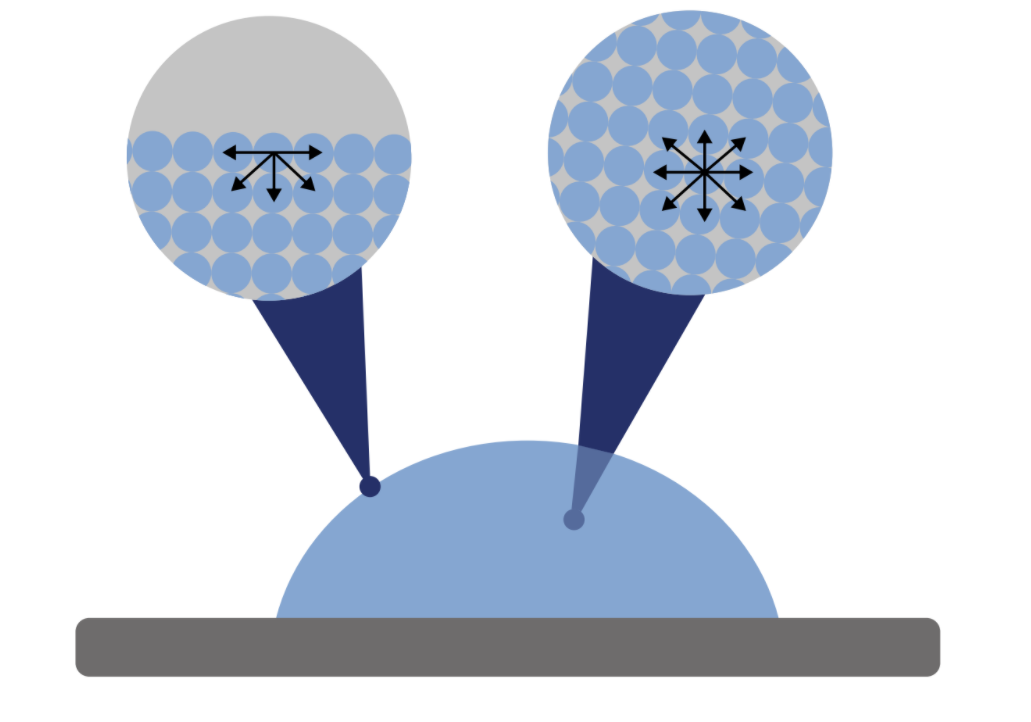
\includegraphics[scale=0.2]{../figs/VN10-PH-46-L-0341-2.png}
\end{center}

Sự hình thành lực căng bề mặt của chất lỏng là do lực tương tác giữa các phân tử của chất lỏng:
\begin{itemize}
	\item Bên trong lòng chất lỏng, các phân tử chất lỏng ở cạnh nhau và phân bố đều theo mọi hướng, nên lực tương tác giữa các phân tử chất lỏng phân bố đều cho các phân tử chất lỏng xung quanh;
	\item Ở bề mặt chất lỏng, các phân tử chất lỏng không phân bố đều theo mọi hướng, nên lực liên kết giữa các phân tử không phân bố đều cho các phân tử xung quanh, do đó hợp lực tác dụng lên mỗi phân tử luôn có xu hướng kéo nó vào trong lòng chất lỏng. 
\end{itemize}
\subsubsection{Một số ví dụ về hiện tượng căng bề mặt của chất lỏng}
\begin{itemize}
	\item Nhờ có lực căng mặt ngoài nên nước mưa không thể lọt qua các lỗ nhỏ giữa các sợi vải căng trên ô dù hoặc trên các mui bạt ô tô;
	\item Hòa tan xà phòng vào nước sẽ làm giảm đáng kể lực căng mặt ngoài của nước nên xà phòng dễ thấm vào các sợi vải khi giặt;
	\item Một giọt nước có trọng lượng rất nhỏ đọng trên chiếc lá sẽ có dạng hình cầu;
	\item Lực căng bề mặt của chất lỏng tạo ra một lớp màng mỏng ngăn những vật có trọng lượng nhỏ (con nhện nước, chiếc kim, $\ldots$) xuyên qua, giúp cho những vật này không bị chìm trong nước.
\end{itemize}

\subsubsection{Công thức tính áp suất của chất lỏng}
\begin{minipage}[l]{0.75\linewidth}
	Áp suất của chất lỏng tại một vị trí có độ sâu $h$ trong lòng chất lỏng:
	$$p = p_0 + \rho g h$$
	
	Trong đó:
	\begin{itemize}
		\item $p_0$ là áp suất khí quyển;
		\item $\rho$ là khối lượng riêng của chất lỏng;
		\item $g$ là gia tốc trọng trường;
		\item $h$ là độ sâu của điểm xác định áp suất chất lỏng so với mặt thoáng.
	\end{itemize}
\end{minipage}
\begin{minipage}[r]{0.15\linewidth}
	\begin{center}
		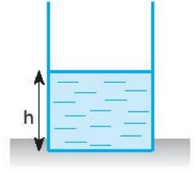
\includegraphics[scale=1]{../figs/G10-029-2}
	\end{center}
\end{minipage}
\subsubsection{Phương trình cơ bản của chất lỏng đứng yên}
Độ chênh lệch áp suất $\Delta p$ giữa 2 điểm M, N có độ sâu lần lượt là $h_1$, $h_2$ chênh lệch nhau $\Delta h$ so với mặt thoáng của chất lỏng đứng yên:

$$\Delta p = \rho g \Delta h$$
\section{Mục tiêu bài học - Ví dụ minh họa}
\begin{dang}{Nắm được định nghĩa khối lượng riêng }
	\viduii{1}{Dựa vào các tài liệu và Internet, em hãy xác định khối lượng riêng của các chất sau: 
		
		\begin{center}
			
			\begin{tabular}{|c|c|c|c|c|c|}
				\hline
				Chất rắn & $\rho$ ($\SI{}{kg/m^3}$)        & Chất lỏng & $\rho$ ($\SI{}{kg/m^3}$) & Chất khí & $\rho$ ($\SI{}{kg/m^3}$) \\ \hline
				Chì      &  & Thủy ngân &     & Carbonic &      \\ \hline
				Đồng     &   & Nước      &       & Oxygen   &      \\ \hline
				Thép     &  & Xăng      &      & Hydrogen &      \\ \hline
			\end{tabular}
			
		\end{center}
	}
	{	\begin{center}
			\textbf{Hướng dẫn giải}
		\end{center}
		
		\begin{center}
			
			\begin{tabular}{|c|c|c|c|c|c|}
				\hline
				Chất rắn & $\rho$ ($\SI{}{kg/m^3}$)        & Chất lỏng & $\rho$ ($\SI{}{kg/m^3}$) & Chất khí & $\rho$ ($\SI{}{kg/m^3}$) \\ \hline
				Chì      & $\SI{11300}{}$ & Thủy ngân &   $\SI{13500}{}$     & Carbonic &    $\SI{1.98}{}$    \\ \hline
				Đồng     & $\SI{8900}{}$  & Nước      &   $\SI{999}{}$     & Oxygen   &  $\SI{1.43}{}$      \\ \hline
				Thép     & $\SI{}{kW}$ & Xăng      &    $\SI{700}{}$    & Hydrogen &   $\SI{0.09}{}$     \\ \hline
			\end{tabular}
			
		\end{center}
	}
	\viduii{2}{Tại sao khối lượng riêng của một chất lại phụ thuộc vào nhiệt độ?
	}
	{	\begin{center}
			\textbf{Hướng dẫn giải}
		\end{center}
		
		Khi nhiệt độ thay đổi, một lượng chất sẽ bị nở ra hoặc co lại, do đó thể tích của chất thay đổi. Trong khi đó, khối lượng của lượng chất đó không thay đổi, vì vậy khối lượng riêng của chất thay đổi:
		$$\text{Khối lượng riêng} = \dfrac{\text{Khối lượng}}{\text{Thể tích}}$$
		
	}
\end{dang}
\begin{dang}{Vận dụng công thức áp suất dựa vào áp lực và diện tích bị ép}
	\viduii{2}{Tại sao xe tăng nặng hơn ô tô nhiều lần lại có thể chạy bình thường trên đất bùn, còn ô tô bị lún và sa lầy trên chính quãng đường này?
	}
	{	\begin{center}
			\textbf{Hướng dẫn giải}
		\end{center}
		
		Mặc dù xe tăng nặng hơn ô tô, do xe tăng có bánh xích nên diện tích xe tăng ép lên mặt đất lớn hơn rất nhiều lần so với diện tích  ô tô ép lên mặt đất, do đó áp suất do xe tăng tác dụng lên mặt đất nhỏ hơn.
		
		Nhờ áp suất lên mặt đất nhỏ, xe tăng có thể chạy bình thường trên đất bùn, còn ô tô bị lún và sa lầy trên chính quãng đường này.
	}
	\viduii{3}{Một người nặng $\SI{50}{kg}$ đứng trên mặt đất nằm ngang. Biết diện tích tiếp xúc của mỗi bàn chân với đất là $\SI{0,015}{m}^2$. Tính áp suất người đó tác dụng lên mặt đất khi:
		\begin{enumerate}[label=\alph*)]
			\item Đứng cả hai chân.
			\item Đứng một chân.
		\end{enumerate}
	}
	{	\begin{center}
			\textbf{Hướng dẫn giải}
		\end{center}
		
		Áp lực của người lên mặt đất đúng bằng trọng lượng người đó:
		$$F=P = mg = \SI{490}{N}$$
		
		\begin{enumerate}[label=\alph*)]
			\item 
			Khi đứng hai chân thì áp suất người đó tác dụng lên mặt đất là
			
			$$p = \dfrac{F}{2S} =\dfrac{mg}{2S}= \SI{16333,34}{N/m}^2.$$
			
			\item 
			Khi đứng một chân thì áp suất người đó tác dụng lên mặt đất là 
			
			$$p = \dfrac{F}{S} = \dfrac{mg}{S} = \SI{32667,67}{N/m}^2.$$
		\end{enumerate}
		
	}
\end{dang}
\begin{dang}{Vận dụng công thức tính áp suất chất lỏng}
	\viduii{2}{Một bình hình trụ cao $\SI{1,8}{m}$ đựng đầy rượu. Biết khối lượng riêng của rượu là $\SI{800}{kg/m}^3$. Áp suất của rượu tác dụng lên điểm M cách đáy bình $\SI{20}{cm}$ là
		\begin{mcq}(4)
			\item $\SI{1440}{Pa}$.
			\item $\SI{1280}{Pa}$.
			\item $\SI{12800}{Pa}$.
			\item $\SI{1600}{Pa}$.
		\end{mcq}
	}
	{	\begin{center}
			\textbf{Hướng dẫn giải}
		\end{center}
		
		Khoảng cách từ điểm M đến mặt thoáng:
		$$h =\SI{1.8}{m} - \SI{0.2}{m} =\SI{1,6}{m}.$$
		
		Áp suất của rượu tác dụng lên M là
		
		$$ p_\text{M} = \rho g h =\SI{12800}{Pa}.$$
		
		\textbf{Đáp án: C}.
	}
	
	\viduii{3}{Một bình hình trụ cao $\SI{0,6}{m}$ chứa lượng nước bằng một nửa chiều cao bình. Biết khối lượng riêng của nước là $\SI{1000}{kg/m}^3$. Áp suất (toàn phần) tác dụng lên điểm M tại đáy bình là bao nhiêu?
	}
	{	\begin{center}
			\textbf{Hướng dẫn giải}
		\end{center}
		
		Khoảng cách từ điểm M đến mặt thoáng:
		$$h =\dfrac{\SI{0.6}{m}}{2}=\SI{0.3}{m}$$
		
		Áp suất khí quyển: $p_0 = \SI{1e5}{N/m^2}$
		
		Áp suất tác dụng lên điểm M tại đáy bình:
		$$ p_\text{M} = p_0 + \rho g h =\SI{103000}{Pa}.$$
		
	}
\end{dang}
\section{Trắc nghiệm}
\begin{enumerate}[label=\bfseries Câu \arabic*:]
	\item \mkstar{1}
	
	
	{
		Trường hợp nào sau đây áp lực của người lên mặt sàn là lớn nhất?
		\begin{mcq} 
			\item Người đứng cả 2 chân.
			\item Người đứng một chân.
			\item Người đứng cả 2 chân nhưng cúi người xuống.
			\item Người đứng cả 2 chân nhưng tay cầm quả tạ.
		\end{mcq}
	}
	
	\hideall
	{	
		\textbf{Đáp án: D.}
		
		Vì áp lực của người lên mặt sàn lớn nhất khi áp lực càng mạnh nên người đứng cả 2 chân nhưng tay cầm quả tạ sẽ tạo ra áp lực lớn hơn các trường hợp còn lại.
		
	}
	\item \mkstar{1}
	
	
	{
		 Trong các cách tăng, giảm áp suất sau đây, cách nào \textbf{không} đúng?
		\begin{mcq}
			\item Muốn tăng áp suất thì tăng áp lực, giảm diện tích bị ép.
			\item Muốn tăng áp suất thì giảm áp lực, tăng diện tích bị ép.
			\item Muốn giảm áp suất thì phải giảm áp lực, giữ nguyên diện tích bị ép.
			\item Muốn giảm áp suất thì phải giữ nguyên áp lực, tăng diện tích bị ép.
		\end{mcq}
	}
	
	\hideall
	{	
		\textbf{Đáp án: B.}
		
		Vì ta có công thức tính áp suất: $p = \dfrac{F}{S}$ nên muốn tăng áp suất thì tăng áp lực, giảm diện tích bị ép. 
	}
	\item \mkstar{1}
	
	
	{Điều nào sau đây đúng khi nói về áp suất chất lỏng?
		\begin{mcq}
			\item Chất lỏng gây áp suất theo mọi phương.
			\item Áp suất tác dụng lên thành bình không phụ thuộc diện tích bị ép.
			\item Áp suất gây ra do trọng lượng của chất lỏng tác dụng lên một điểm tỉ lệ nghịch với độ sâu.
			\item Nếu cùng độ sâu thì áp suất như nhau trong mọi chất lỏng khác nhau.
		\end{mcq}
	}
	
	\hideall
	{	
		\textbf{Đáp án: A.}
		
		Chất lỏng gây áp suất theo mọi phương lên đáy bình, thành bình và các vật ở trong lòng nó
	}
	\item \mkstar{1}
	
	
	{Áp suất mà chất lỏng tác dụng lên một điểm phụ thuộc:
		\begin{mcq}
			\item Khối lượng lớp chất lỏng phía trên.
			\item Trọng lượng lớp chất lỏng phía trên.
			\item Thể tích lớp chất lỏng phía trên.
			\item Độ cao lớp chất lỏng phía trên.
		\end{mcq}
	}
	
	\hideall
	{	
		\textbf{Đáp án: D.}
		
		Áp suất mà chất lỏng tác dụng lên một điểm phụ thuộc độ cao lớp chất lỏng phía trên.
	}

\end{enumerate}
\hideall
{
	\begin{center}
		\textbf{BẢNG ĐÁP ÁN}
	\end{center}
	\begin{center}
		\begin{tabular}{|m{2.8em}|m{2.8em}|m{2.8em}|m{2.8em}|m{2.8em}|m{2.8em}|m{2.8em}|m{2.8em}|m{2.8em}|m{2.8em}|}
			\hline
			1.D  & 2.B  & 3.A  & 4.D  &  &   &  &   &  &   \\
			\hline
		
		\end{tabular}
	\end{center}
}
\section{Tự luận}

\begin{enumerate}[label=\bfseries Câu \arabic*:]

	\item \mkstar{2}
	
	
	{
		Một người nặng $\SI{50}{kg}$ đứng trên mặt đất nằm ngang. Biết diện tích tiếp xúc của mỗi bàn chân với đất là $\SI{0,015}{m}^2$. Tính áp suất người đó tác dụng lên mặt đất khi đứng cả hai chân và khi đứng một chân.
	}
	
	\hideall
	{	
		Khi đứng một chân thì áp suất người đó lên mặt đất là 
		
		$$p = \dfrac{F}{S} = \dfrac{mg}{S} = \SI{32667,67}{N/m}^2.$$
		
		Khi đứng hai chân:
		
		$$p = \dfrac{F}{2S} = \SI{163334,34}{N/m}^2.$$
	}
	\item \mkstar{2}
	
	
	{
		Một khối hình lập phương có cạnh $\SI{0,3}{m}$, chìm $\dfrac{2}{3}$ trong nước. Biết khối lượng riêng của nước là $\SI{1000}{kg/m}^3$. Tính áp suất của nước tác dụng lên mặt dưới của khối lập phương. Lấy $g = \SI{9,8}{m/s}^2.$
	}
	
	\hideall
	{	
		Do khối lập phương chìm $\dfrac{2}{3}$ trong nước nên $ h= \dfrac{2}{3}a$.
		
		Áp suất của nước tác dụng lên khối lập phương là
		
		$$ p = \rho g h = \SI{1960}{N/m}^2.$$
		
		
	}
	
	\item \mkstar{3}
	
	
	{
		Một xe tải 6 bánh có khối lượng 8 tấn, diện tích tiếp xúc của mỗi bánh xe với mặt đất là $\SI{7,5}{cm}^2$. Tính áp suất của xe lên mặt đường khi xe đứng yên
	}
	
	\hideall
	{	
		Trọng lượng của vật là
		$$P = mg = \SI{80000}{N}.$$
		
		Áp suất của xe tải tác dụng lên mặt đường là: $$p=\dfrac{F}{6S}=\SI{17777777,8}{N/m^2}.$$
		 
	}
	\item \mkstar{3}
	
	
	{
		Một xe contener có trọng lượng $\SI{26000}{N}$. Tính áp suất của xe lên mặt đường, biết diện tích tiếp xúc với mặt đất là $\SI{130}{dm}^2$. Hãy so sánh áp suất đó với áp suất của một người nặng $\SI{45}{kg}$ có diện tích tiếp xúc 2 bàn chân với mặt đất là $\SI{200}{cm}^2$. Cho $g =\SI{10}{m/s}^2$.
	}
	
	\hideall
	{	
		Áp suất của xe tăng lên mặt đường:
		
		$$p_1=\dfrac{F_1}{S_1}=\SI{21666,67}{Pa}.$$
		
		Áp lực của người lên mặt đất là:
		
		$$P_2=F_2=m_2g=\SI{450}{N}.$$
		
		Áp suất của người lên mặt đất là:
		
		$$p_2=\dfrac{F_2}{S_2}= \SI{22500}{Pa}.$$
		
		$$\Rightarrow p_1 < p_2.$$
		
		Vậy áp suất của người lớn hơn của xe contener.
	}
	\item \mkstar{2}
	
	
	{
		Có hai loại xẻng như hình. Khi tác dụng cùng một lực thì xẻng nào nhấn vào đất được dễ dàng hơn? Tại sao?
		\begin{center}
			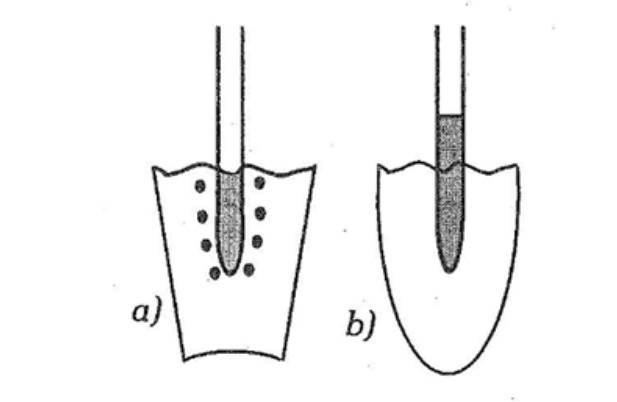
\includegraphics[scale=0.35]{../figs/VN10-2022-PH-TP036-1.jpg}
		\end{center}
		
	}
	
	\hideall
	{	
		Loại xẻng có đầu nhọn nhấn vào đất dễ dàng hơn vì diện tích bị ép nhỏ hơn loại xẻng có đầu bằng, khi tác dụng cùng một áp lực thì áp suất của xẻng có đầu nhọn lớn hơn áp suất của xẻng có đầu bằng.
	}
		\item \mkstar{3}
	
	
	{
		Một hợp kim đồng và bạc có khối lượng riêng là $\SI{10,3}{g/cm}^3$. Tính khối lượng của bạc và đồng có trong $\SI{100}{g}$ hợp kim. Biết khối lượng riêng của đồng là $\SI{8,9}{g/cm}^3$, của bạc là $\SI{10,4}{g/cm}^3$.
	}
	
	\hideall
	{	
		Gọi $m_1, V_1$ lần lượt là khối lượng, thể tích, khối lượng riêng của bạc.
		
		$m_2, V_2$ lần lượt là khối lượng, thể tích, khối lượng riêng của đồng.
		
		Thể tích của khối hợp kim
		
		$$\rho = \dfrac{m}{V} \Rightarrow V = \dfrac{m}{\rho} = \dfrac{1000}{103}\ \text{cm}^3.$$
		
		Thể tích của khối hợp kim bằng thể tích của bạc và đồng có trong hợp kim.
		
		Ta có: $$V = V_1 + V_2 \Rightarrow V = \dfrac{m_1}{\rho_1} + \dfrac{m_2}{\rho_2}$$ 
		
		Với $m = m_1 + m_2 = \SI{100}{g}.$
		
		Thay số vào ta được:
		
		$$\dfrac{1000}{103} = \dfrac{m_1}{\text{10,4}} + \dfrac{100 - m_1}{\text{8,9}} \Rightarrow m_1 \approx \SI{94,24}{g} \Rightarrow m_2 \approx \SI{5,76}{g}.$$
		
		
		Vậy khối lượng của bạc là $\SI{94,24}{g}$; khối lượng của đồng là $\SI{5,76}{g}.$
	}
\end{enumerate}